\documentclass[final]{beamer}
\usepackage[size=a0,scale=1.0]{beamerposter}
\usepackage{graphicx}
\usepackage{amsmath, amssymb}
\usepackage{tikz}
\usepackage{qrcode}
\usepackage{blkarray} % optional for QR codes

\title{Cross-Platform Quantum Compiler for Hamiltonian Decomposition}
\author{Shoupu Wan}
\institute{Quantum Simulations Project — GitHub: \texttt{wanshoupu/quantum-simulations}}

\begin{document}

\begin{frame}[t]

  \begin{columns}[t]

    % Column 1
    \begin{column}{0.33\textwidth}
      \begin{block}{Motivation}
        Most quantum compilers are tied to specific hardware. Our compiler bridges that gap, allowing...
      \end{block}

      \begin{block}{Theory}
        We consider a general Hamiltonian \( H = \sum_i \alpha_i P_i \) where \( P_i \) are Pauli strings...
      \end{block}
    \end{column}

    % Column 2
    \begin{column}{0.33\textwidth}
      \begin{block}{Architecture}
        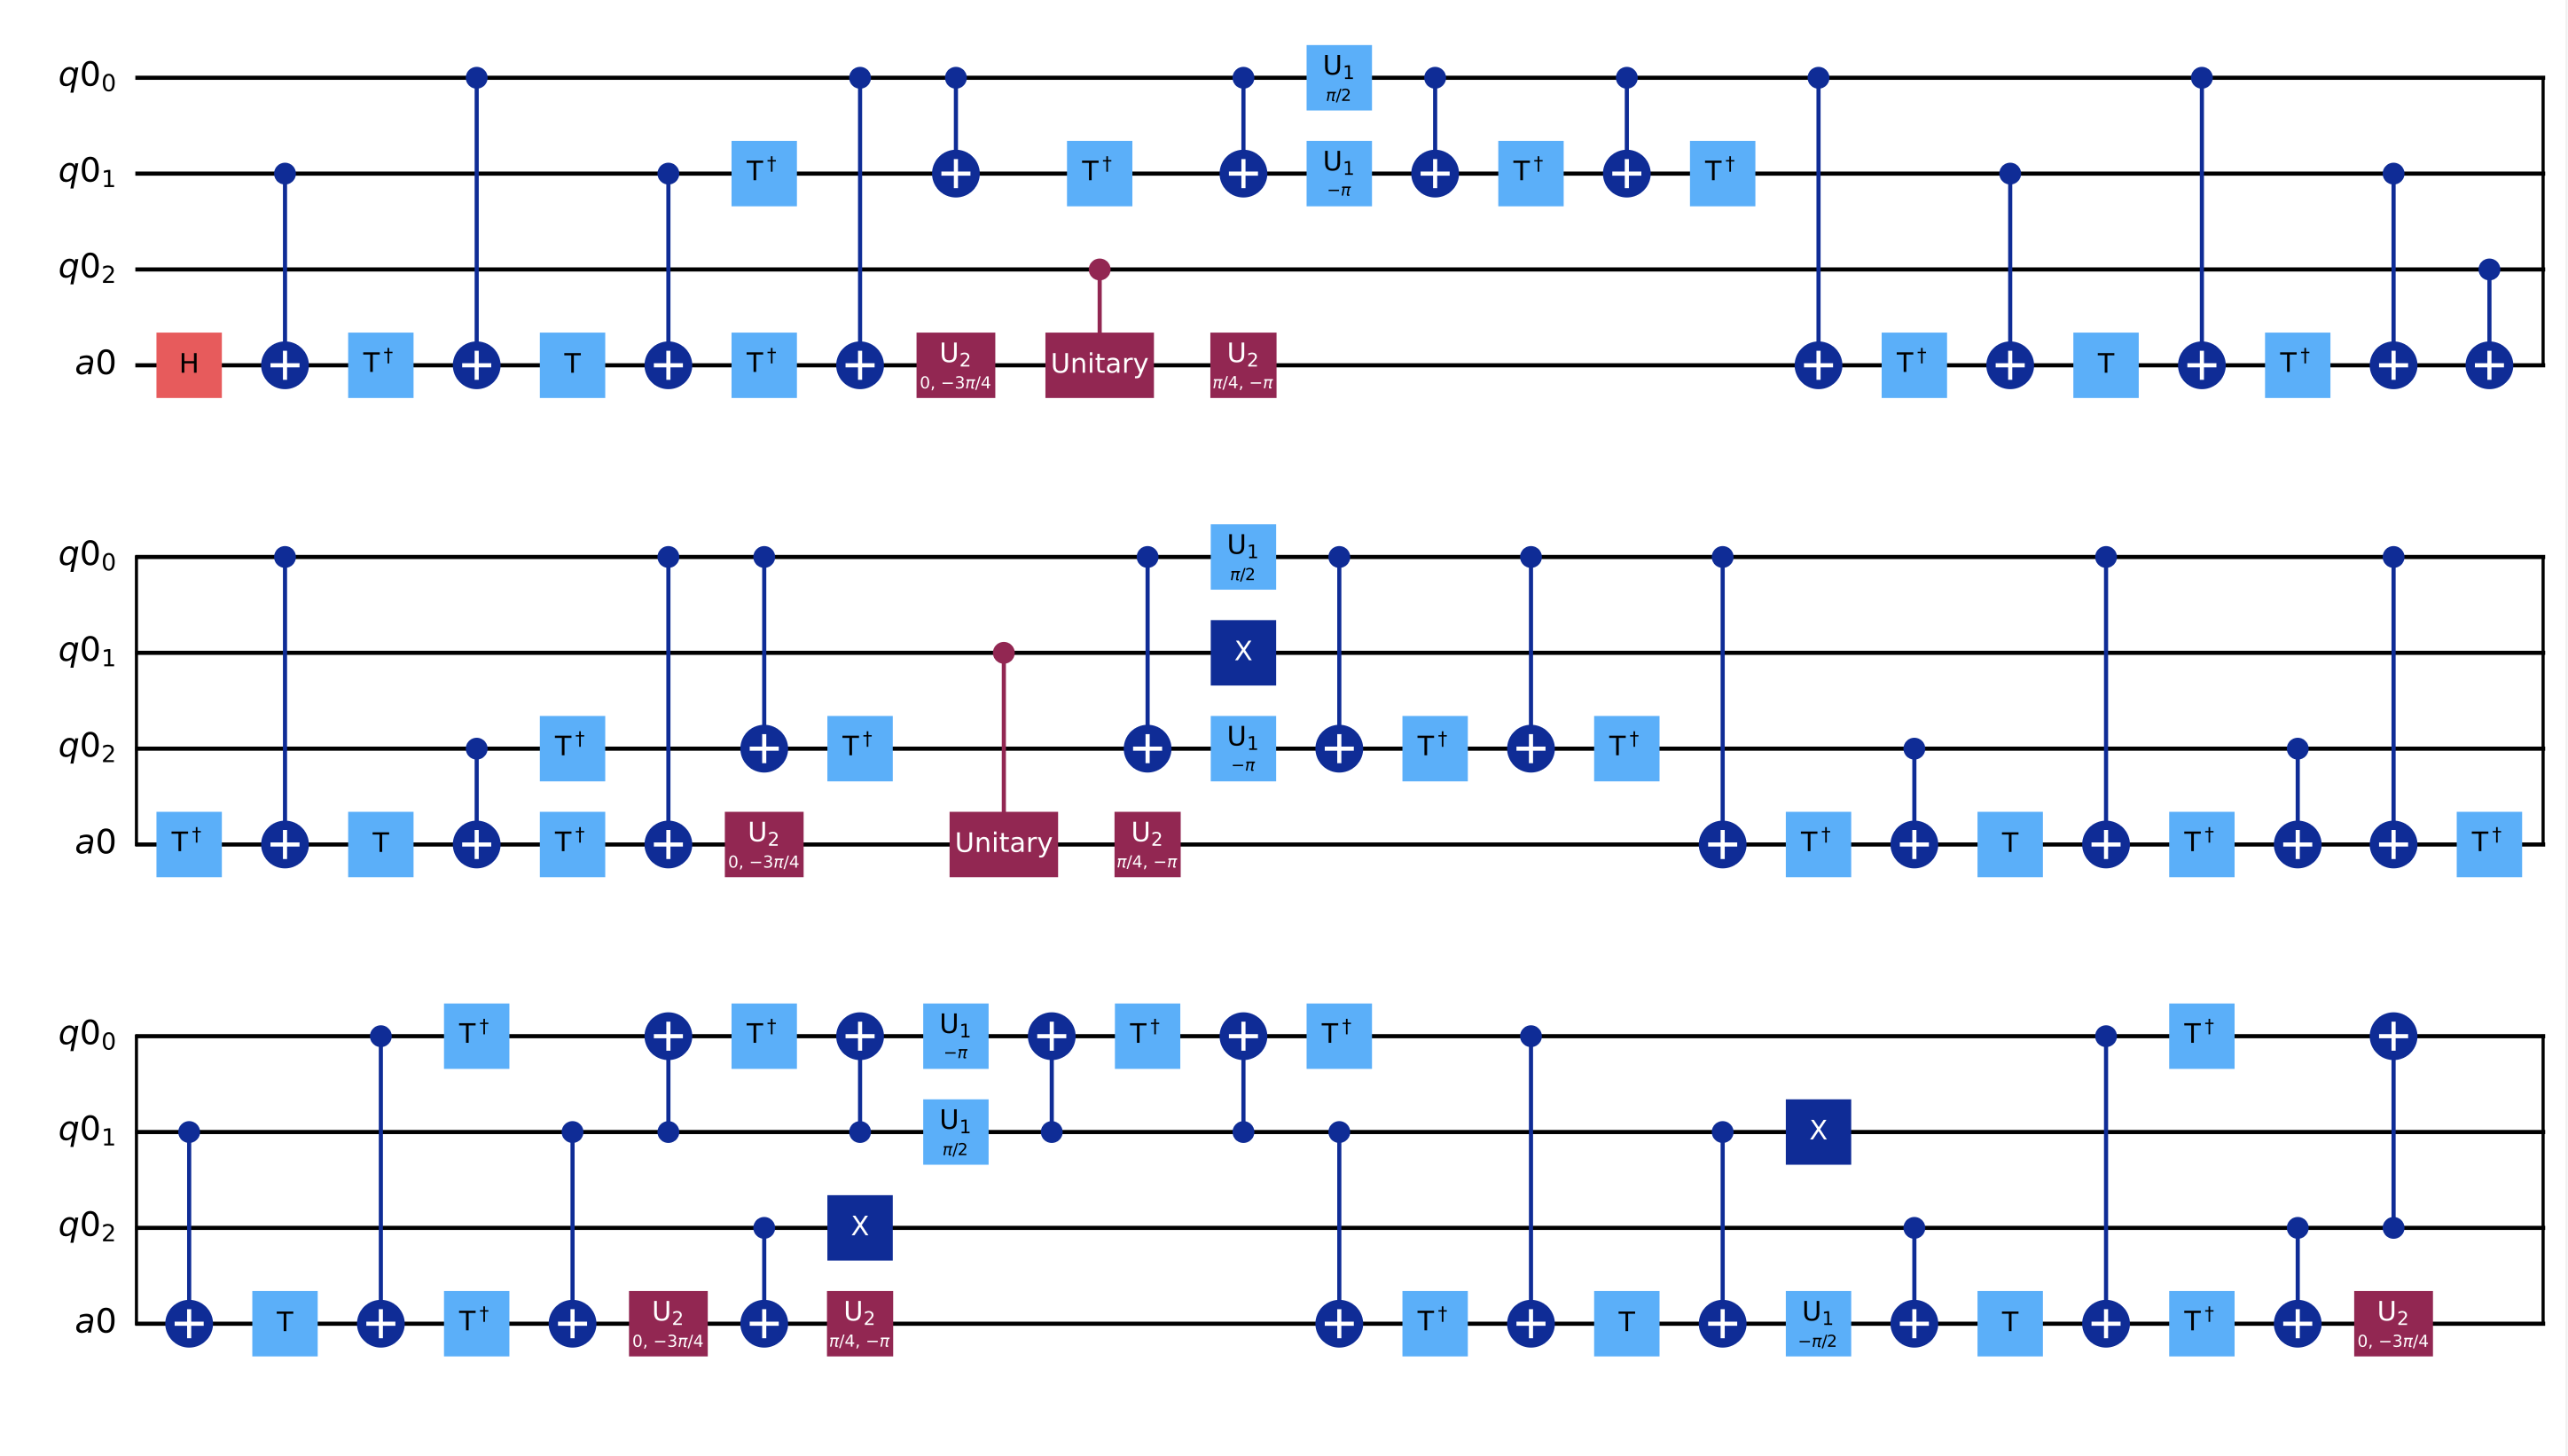
\includegraphics[width=\linewidth]{compiler-architecture.png}

        Pipeline: Parse → Decompose → Synthesize → Target Platform
      \end{block}

      \begin{block}{Platforms Supported}
        \begin{itemize}
          \item Cirq
          \item Qiskit
          \item AWS Braket (coming)
          \item PennyLane (planned)
        \end{itemize}
      \end{block}
    \end{column}

    % Column 3
    \begin{column}{0.33\textwidth}
      \begin{block}{Demo}
        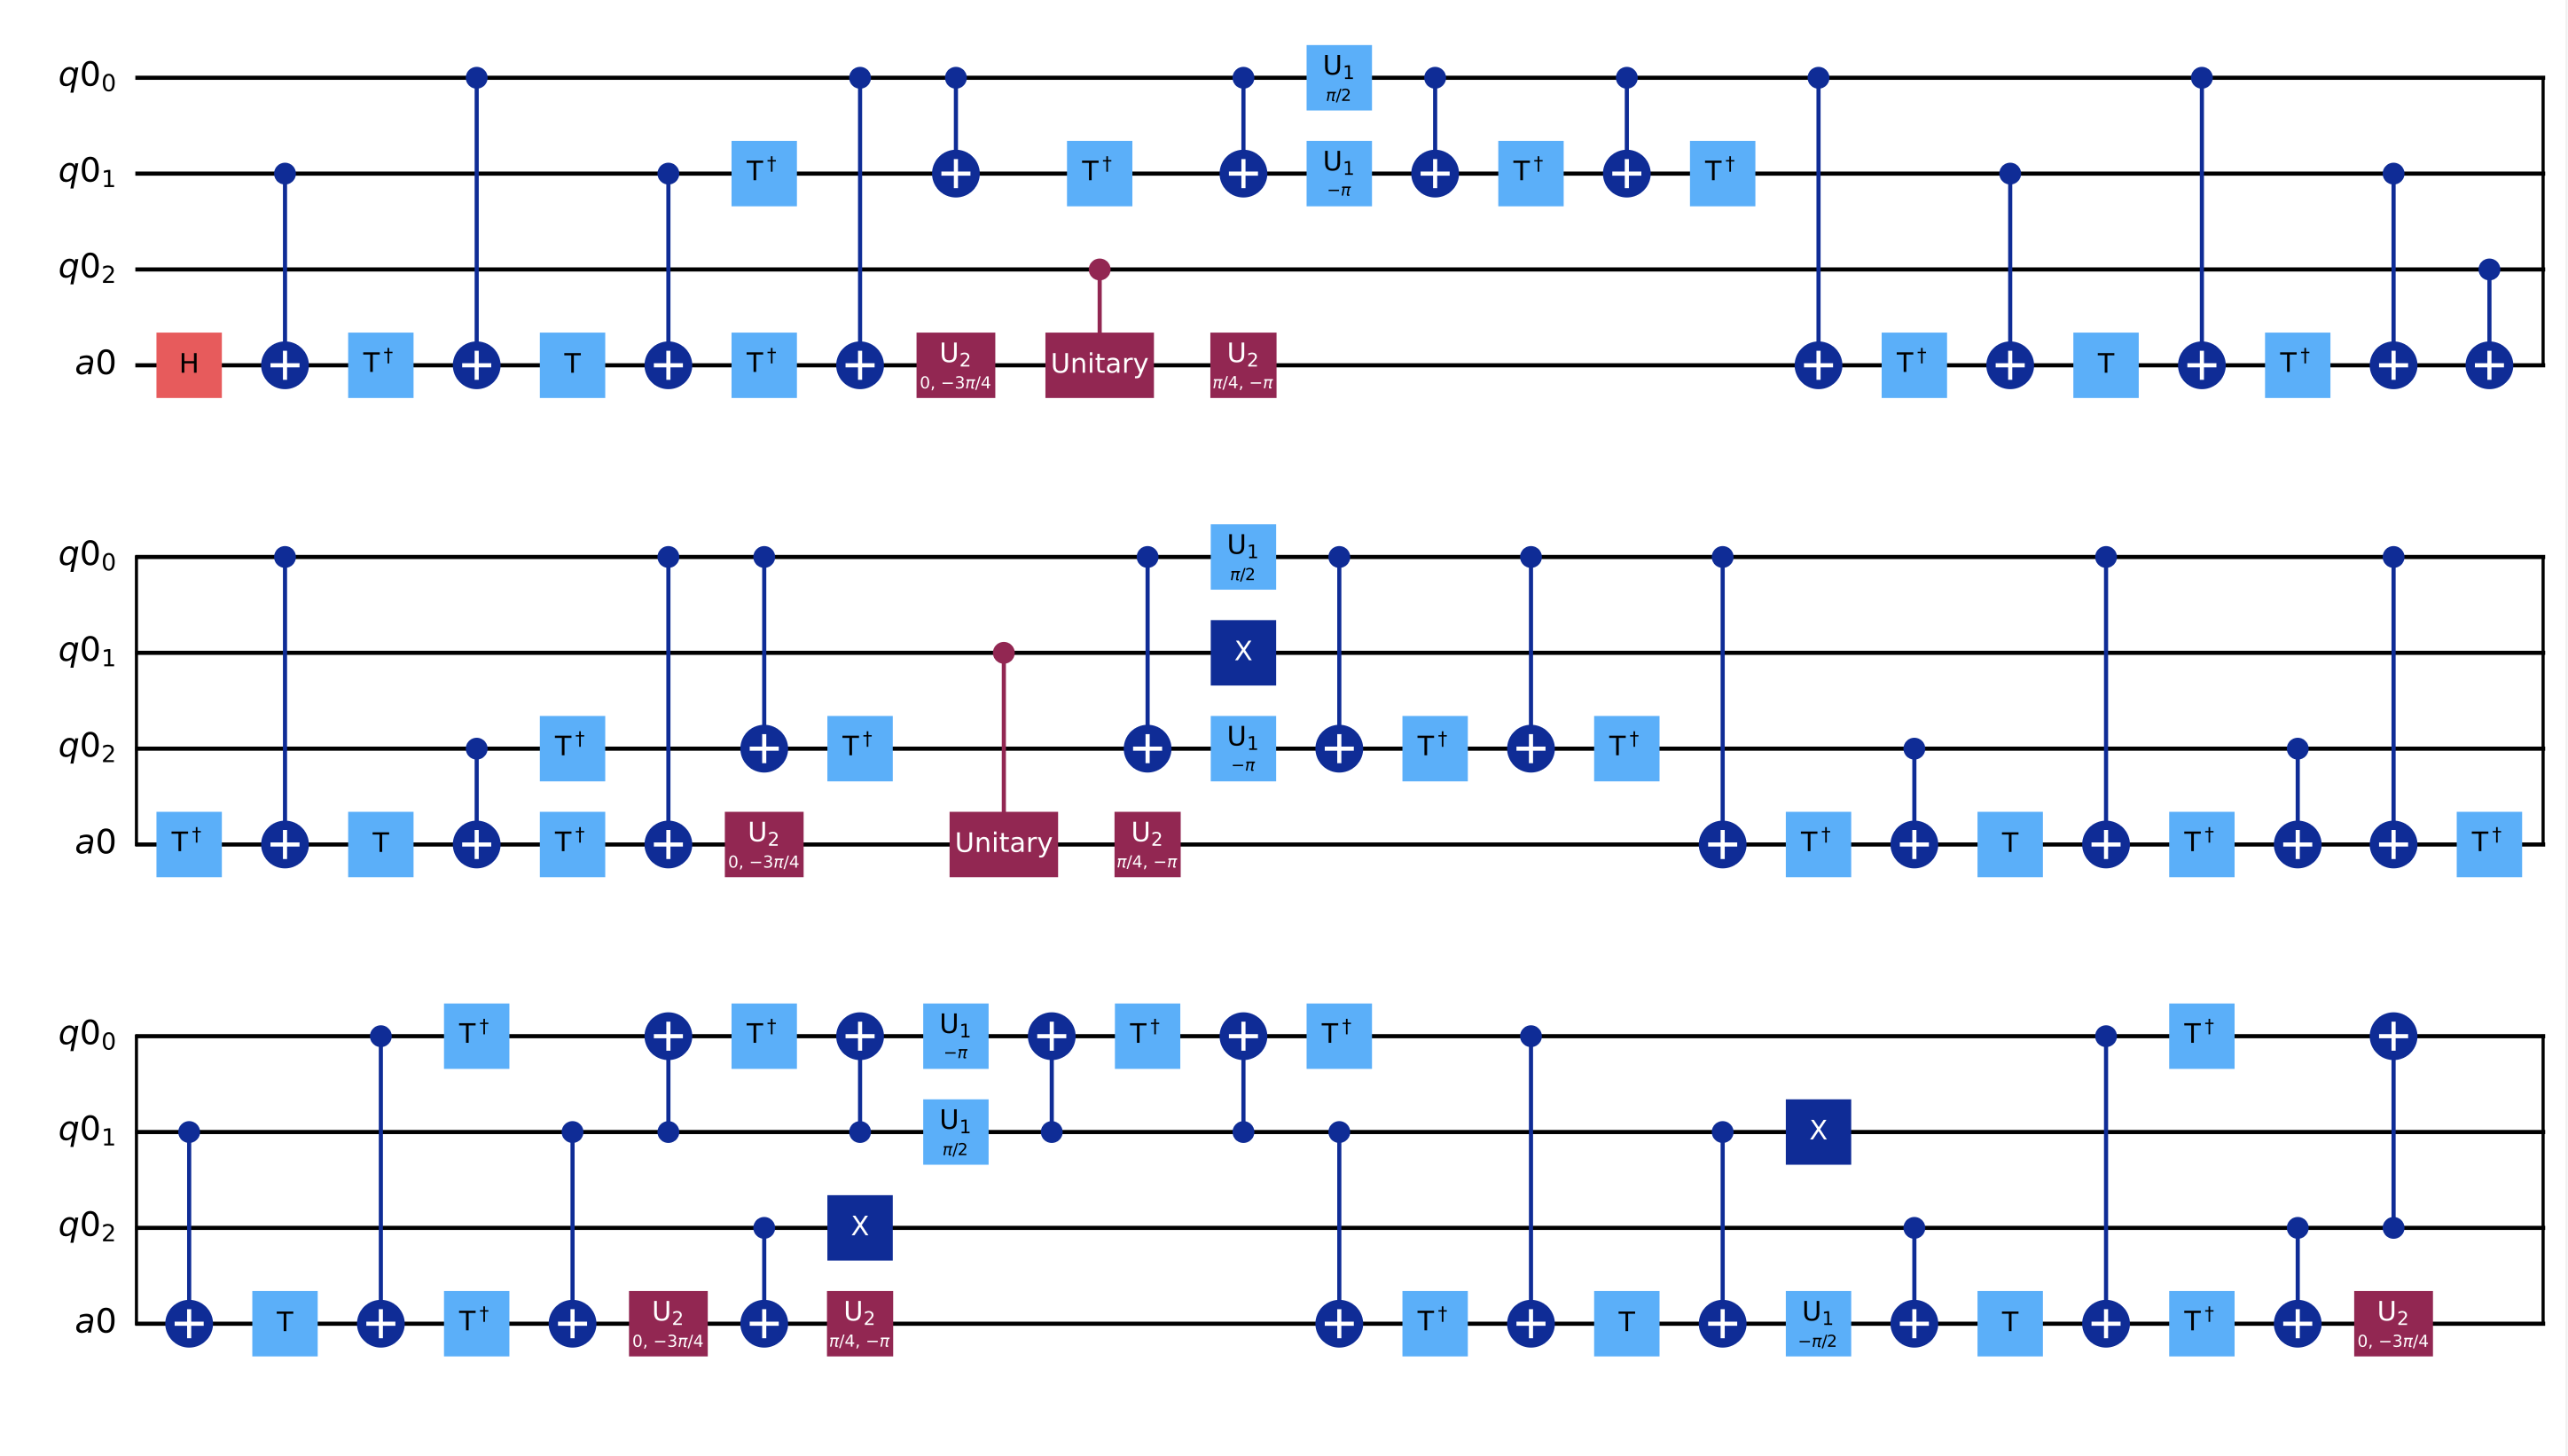
\includegraphics[width=\linewidth]{circuit-example.png}
      \end{block}

      \begin{block}{Get the Code}
        \qrcode{https://github.com/wanshoupu/quantum-simulations}

        \vspace{1em}
        \texttt{github.com/wanshoupu/quantum-simulations}
      \end{block}

      \begin{block}{Conclusion}
        This tool helps democratize quantum simulation and hardware mapping.
        \textbf{Feedback and collaboration welcome!}
      \end{block}
    \end{column}

  \end{columns}

\end{frame}

\end{document}
